\documentclass{beamer}

\usepackage{amssymb}
\usepackage{fancyvrb}
\usepackage{stmaryrd}
\usepackage{graphicx}
\usepackage{tikz}
\usefonttheme{serif}


\newcommand{\Nat}{\mathbb{N}}

\title{Data Science}%\texorpdfstring{$\mathbb{N}$}}
\subtitle{\blueit{Introduction to Machine Learning:\\
                  Decision Trees. Overfitting.}}
\date{April 19, 2021}

\usetheme{jmct}

\usepackage{calc}

\newcommand{\textover}[3][l]{%
 % #1 is the alignment, default l
 % #2 is the text to be printed
 % #3 is the text for setting the width
 \makebox[\widthof{#3}][#1]{#2}%
 }

\newcommand{\blueit}[1]{%
  {\color{dark-lucid-blue}#1}%
}
\newcommand{\blueite}[1]{%
  \blueit{\emph{#1}}%
}
\newcommand{\redit}[1]{%
  {\color{my-magenta}#1}%
}


\newcommand{\myquote}[3]{
  ``#1''
  \vspace{3pt}
  \hrule
  \begin{flushright}
  --- \blueit{\emph{#2}}, \emph{#3}
  \end{flushright}
}

\begin{document}
	\frame {
		\titlepage
	}

\newcommand{\withwidth}[2]{%
  \makebox[\widthof{#2}][c]{#1}%
}

%%%%%%%%%%%%%%%%%%%%%%%%%%%%%%%%%%%%%%%% 
%%% Intro
%%%%%%%%%%%%%%%%%%%%%%%%%%%%%%%%%%%%%%%% 

  \frame{
    \frametitle{Recap on the general problem}
    Many Machine Learning problems take the following form:

    \begin{equation*}
    \text{minimize}_\theta ~ \sum_{i=1}^{m} l(h_{\theta}(x^{(i)}), y^{(i)})
    \end{equation*}

    \vspace{0.5cm}
    \onslide<2 ->{We've now looked at some $l$s and an $h$.}
  }

  \frame{
    \frametitle{Previously, on...}
    Hypothesis function
    \begin{enumerate}
      \item<2 -> We looked at a linear regression
      \item<3 -> We `fit' this linear regression to our dataset
      \item<4 -> If our data is actually linear, we also get \emph{predictive} power
    \end{enumerate}
  }

  \frame{
    \frametitle{A wild $h$ appears}
    Linear Regressions aren't the only possible hypothesis function! We've also got:
      \begin{enumerate}
        \item<2 -> \blueite{\withwidth{Decision Trees}{Arbitrary Programs}}: 20-questions, the ML technique
        \item<3 -> \blueite{\withwidth{Polynomials}{Arbitrary Programs}}: For when a straight line isn't cutting it
        \item<4 -> \blueite{\withwidth{Neural networks}{Arbitrary Programs}}: What if we misunderstood neurons and made it a program?
        \item<5 -> \blueite{Arbitrary Programs}: What is computers wrote the programs?
      \end{enumerate}
  }

  \frame{
    \frametitle{Do you realize?}

    A learning problem is said to be \blueite{realizable} if the \redit{true function} exists within
    the learning problem's \blueite{hypothesis space} 

      \begin{enumerate}
        \item<2 -> This means that the more \blueit{expressive} the hypothesis space (polynomials vs straight lines) the more likely that the problem is realizable.
        \item<3 -> What's the downside?
        \item<4 -> Occam's\footnote{\onslide<4->{Also written as `Ockham' or `Ocham'}} Razor is a data-scientist's best friend
      \end{enumerate}
  }

%%%%%%%%%%%%%%%%%%%%%%%%%%%%%%%%%%%%%%%% 
%%% Decision Trees
%%%%%%%%%%%%%%%%%%%%%%%%%%%%%%%%%%%%%%%% 


  \frame{
    \frametitle{Decision Trees}
      We can view our tagged dataset (values of $(x, tag)$), as standing in for values of $(x, f(x))$.
      
      \begin{enumerate}
        \item<2 -> As with the linear regression the goal is to find an $h$ that \blueit{approximates} $f$.
        \item<3 -> But instead of a regression, we want a \redit{tree} of \blueite{decisions}.
        \item<4 -> What's a decision?
      \end{enumerate}
  }

  \frame{
    \frametitle{Decisions! Decisions!}
    Each decision has two parts:

      \begin{enumerate}
        \item<2 -> \blueite{\withwidth{Input}{Output}}: An object\footnote{not in the OO sense} event/situation, that is described by a set of attributes (or \emph{features})
        \item<3 -> \blueite{\withwidth{Output}{Output}}: A prediction of the `value' based on the input
        \item<4 -> The boolean case (yes/no) is easy to visualize, but the values do not have to be discrete.
      \end{enumerate}
  }

  \frame{
    \frametitle{Consider}
    You are asked to identify an animal based on a set of features (number of legs, weight, number of eyes, etc.)

      \begin{enumerate}
        \item<2 -> The challenge is that the \emph{order} of questions can matter!
        \item<3 -> You'll want the 'most significant' question first.
        \item<4 -> Unfortunately, it can be very expensive(!!) to find the most significant question.
      \end{enumerate}
  }

  \frame{
    \frametitle{A tiny bit more formally:}
    A decision tree has two types of nodes:

      \begin{enumerate}
        \item<2 -> Decision nodes: Specifies a test on some attribute
        \item<3 -> Leaf node: A final classification/prediction
      \end{enumerate}
  }

  \frame{
    \frametitle{Small example:}
    We want to determine whether someone has ever seen an episode of Sponge Bob:

      \begin{enumerate}
        \item<2 -> Are they older than 70: no.
        \item<3 -> Are they older then 40: if yes...
          \begin{enumerate}
            \item<4 -> Do they have kids: if yes, yes.
            \item<5 -> no.
          \end{enumerate}
        \item<6 -> Are they older than 4: yes.
        \item<7 -> Do they have older siblings: yes.
        \item<8 -> no.
      \end{enumerate}
  }

  \frame{
    \frametitle{Oof}
    Even for such a small example, it starts getting unwieldy.

      \begin{enumerate}
        \item<2 -> Luckily, libraries will be able to display trees nicely
        \item<3 -> For many trees it's not necessarily true that each `decision', will have a meaningful-in-English question associated with it.
      \end{enumerate}
  }

  \frame{
    \frametitle{A prettier example}
    Should we wait for a table?

    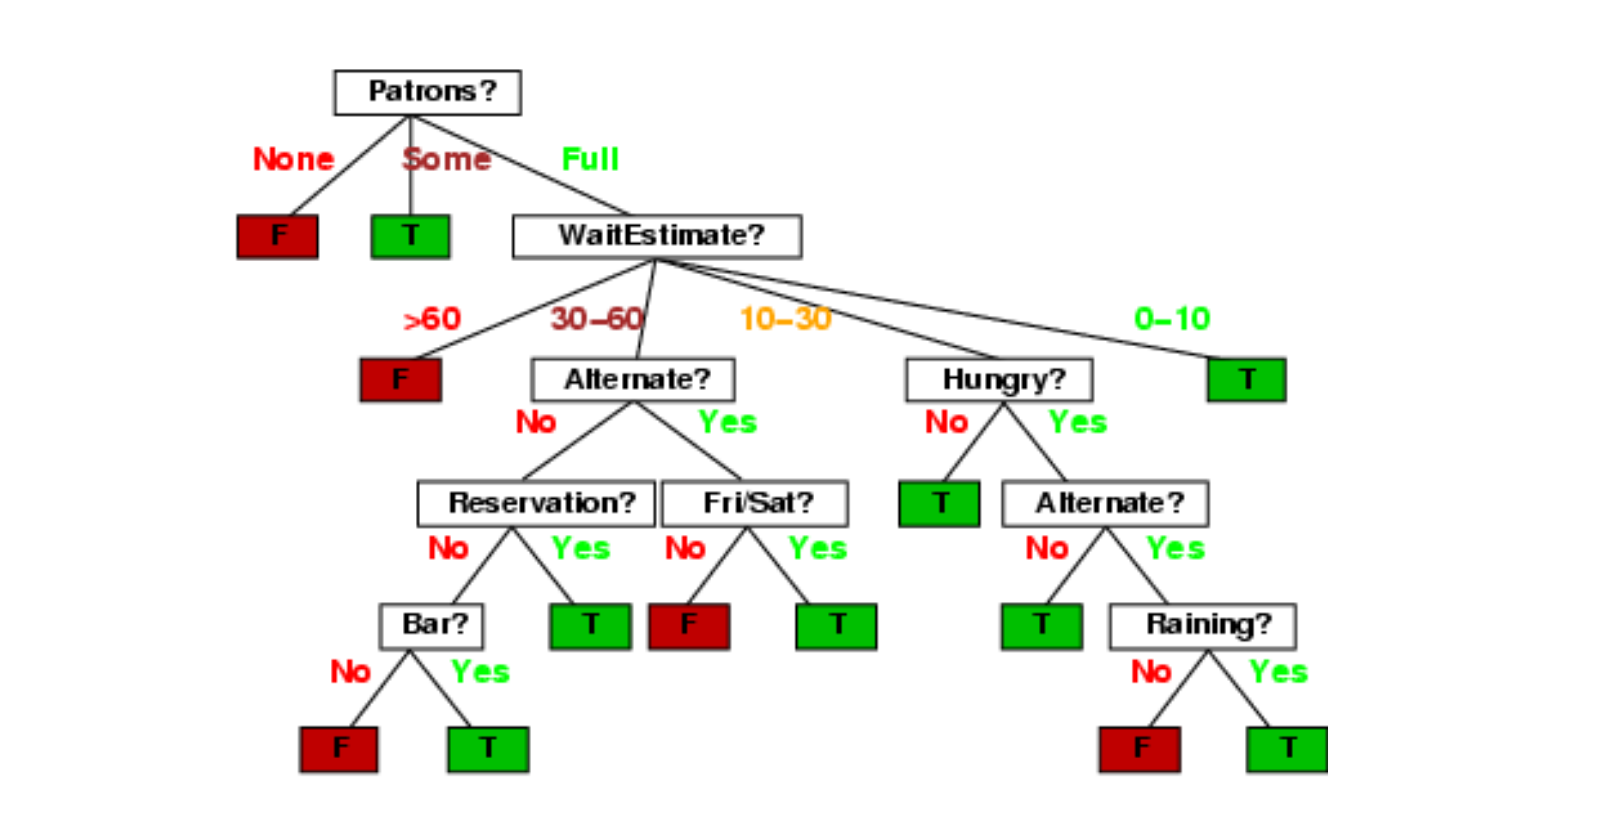
\includegraphics[width=\textwidth]{figs/dt1.png}
  }

  \frame{
    \frametitle{How many are there?}
    Decision Trees can encode arbitrary boolean functions.

      \begin{enumerate}
        \item<2 -> Each attribute can be 0/1
        \begin{enumerate}
          \item<3 -> So our \emph{input} space is $2^N$
        \end{enumerate}
        \item<4 -> Each decision value can be 0/1, \emph{for each possible combination of features!}
        \begin{enumerate}
          \item<5 -> So our \emph{hypothesis space} is $2^{2^N}$
        \end{enumerate}
      \end{enumerate}
  }

  \frame{
    \frametitle{Basic Algorithm}
    The goal is to find a \emph{small} tree that correctly predicts the training samples

      \begin{enumerate}
        \item<2 -> Choose the ``most significant'' attribute
        \item<3 -> Once you make a choice for ``most significant'', you don't backtrack (greedy)
        \item<4 -> Now you've split your dataset, repeat the process for each subset.
      \end{enumerate}
  }


  \frame{
    \frametitle{Significant?}
    How do we pick the ``most significant''?

      \begin{enumerate}
        \item<2 -> We can't always :(
        \item<3 -> We want to try and maximize \emph{information gain}
        \item<4 -> For this class: let the libraries do the work for you.
      \end{enumerate}
  }

%%%%%%%%%%%%%%%%%%%%%%%%%%%%%%%%%%%%%%%% 
%%% Overfitting
%%%%%%%%%%%%%%%%%%%%%%%%%%%%%%%%%%%%%%%% 

  \frame{
    \frametitle{Fit and Finish}
    For all ML techniques, there's a danger of \blueite{overfitting}.

      \begin{enumerate}
        \item<2 -> What does overfitting imply?
        \item<3 -> How would we know if we've done it?
      \end{enumerate}
  }

  \frame{
    \frametitle{Holdout Cross Validation}
    Idea: Don't use all your training data!

      \begin{enumerate}
        \item<2 -> Instead of training your model on every you have, train it on some subset (training set).
        \item<3 -> Once you have the trained model, you \emph{test} it on the rest, the \blueite{test set} (since you know the classifications).
        \item<4 -> You \emph{must} ensure that your subsets are independent!
      \end{enumerate}
  }

  \frame{
    \frametitle{This slide is a trick}
    Consider:

      \begin{enumerate}
        \item<2 -> We train four different hypothesis functions
        \item<3 -> We use our test set to see which hypothesis function performs best
        \item<4 -> We publish our awesome model!
        \item<5 -> Is the celebration warranted?
      \end{enumerate}
  }



%%%%%%%%%%%%%%%%%%%%%%%%%%%%%%%%%%%%%%%% 
%%% Conclusion
%%%%%%%%%%%%%%%%%%%%%%%%%%%%%%%%%%%%%%%% 

  \frame{
    \frametitle{Thanks for your time!}

     :) 
  }


\end{document}
